\section{Cloud und Edge Robotic Use Cases} % (fold)
\label{sec:Cloud und Edge Robotic Use cases}

Nachdem in den vorangegangenen Abschnitten relevante Technologien und Architekturen rund um das Thema Cloud und Edge Robotics vorgestellt wurden, wird im folgenden auf verschiedene Use Cases eingegangen und wie man sie mit den bereits besprochenen Konzepten realisieren kann. Dabei werden Konzepte wie die der digitalen Zwillinge, dem Nutzen von verschiedenen Schnittstellen oder dem Zugang über entfernte Systeme behandelt die bereits im Cloud und Edge Computing so wie Robotics Bereich eine Rolle spielen.\\

\subsection{Digitale Zwillinge in der Robotik} % (fold)
\label{sub:Digitale Zwillinge in der Robotik}

Das Konzept der digitalen Zwillinge beschreibt die Möglichkeit, virtuelle Abbilder von Objekten aus der physischen Welt zu erzeugen und für verschiedenen Anwendungszwecke zu nutzen \cite{fullerDigitalTwinEnabling2020}. Beispiele hierfür sind das Testen von Software, der Einsatz von Simulationen oder die Leistung im Vorhinein zu verbessern.\\
Die Robotik ist ein interessanter Bereich wenn es um die Anwendung von digitale Zwillingen geht. Roboter können dabei zum Beispiel digital repliziert werden und so einfacher getestet oder gesteuert werden. Im folgenden Use Case, wird eine im Vorhinein aufgenommene Sequenz an Aktionen in einer Datenbank gespeichert. Es wird also eine Simulation der Aktionen die ein Roboter ausführt zuvor aufgenommen um später auf einem oder mehreren Roboter ausgespielt zu werden. Dies kann vor allem in der Industrie nützlich sein, wenn man eine Kontrollierte Umgebung hat die keine externe Faktoren hat die eine Simulation stören könnte. Unternehmen könnten hiermit einzelne oder mehrere Roboter in einer Fabrik automatisiert jederzeit auf eine bestimmte Sequenz von Aufgaben ansetzen und Fehler der Roboter durch weitere Simulation verbessern.\\

Der Aufbau des Use Cases ist in \ref{fig:Digitale Zwillinge in der Robotik} dargestellt. Dafür werden folgende Komponenten benötigt:

\begin{enumerate}
  \item Simulator: Mit diesem ist es möglich, die Aktionen eines Roboters zu simulieren und aufzunehmen. Dieser veröffentlicht die Simulationsdaten an den Zenoh Router. Der Simulator verhält sich dabei wie ein ROS2 System. Aus diesem Grund wird hier noch das Zenoh DDS Plugin genutzt.
  \item Zenoh Router: Um die Daten zwischen den verschiedenen Komponenten auszutauschen und weiterzuleiten wird das Zenoh Protokoll verwendet. Dafür wird ein zentraler Zenoh Router in der Cloud eingesetzt. Dieser nimmt die Daten des Simulators an, leitet eine Speicherung in der Datenbank ein und veröffentlicht diese an einem späteren Zeitpunkt an den Roboter.
  \item Datenbank: In dieser werden die Aktionen gespeichert, die im Roboter eingespielt werden sollen. Diese können zum Beispiel durch das Influx Datenbank Plugin für Zenoh angebunden werden. Influx ist dabei eine ein Datenbank Managementsystem welches auf das speichern von Zeitreihen spezialisiert ist. Dies ist hilfreich, um beim Abrufen der Simulation die Daten in der richtigen Reihenfolge auszugeben. Interessant ist hier ebenfalls die Einbindung mit Zenoh. Wie bei der Beschreibung der Router in Abschnitt \ref{sec:Cloud und Edge Robotic Architekturen} angedeutet, kann man die Datenbank durch ein Zenoh Plugin direkt mit dem Zenoh Router verbinden. Daraufhin ist es dann möglich, alle zu einem Topic (In diesem Fall \code{robot1/rt/cmd\_vel}) gehörenden Daten automatisch in der Datenbank über den Router zu speichern.
  \item Edge Server und Roboter: Um das einspielen der Simulation in den realen Roboter zu ermöglichen, wird ein Edge Server eingesetzt. Wenn die Simulation im Roboter eingespielt werden soll, startet dieser eine Query auf das \code{robot1/rt/cmd\_vel} Topic. Dies löst eine Anfrage in der Datenbank aus, welche die Daten aussendet. Der Edge Server published diese dann nur noch an den Roboter der auf diese subscribed und die Aktionen ausführt.
\end{enumerate}

\begin{figure}
  \begin{center}
    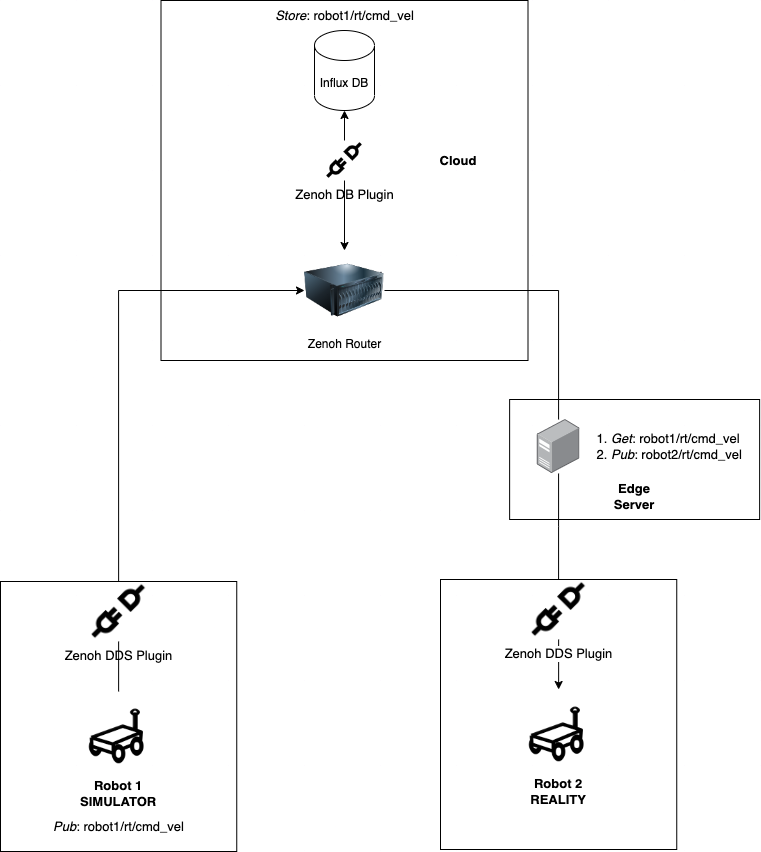
\includegraphics[width=0.6\textwidth]{figures/digitalle-zwillinge.drawio.png}
  \end{center}
  \caption{Digitale Zwillinge in der Robotik}
  \label{fig:Digitale Zwillinge in der Robotik}
\end{figure}

% subsection Digitale Zwillinge in der Robotik (end)

\subsection{Robotersteuerung über den Browser} % (fold)
\label{sub:Robotersteuerung über den Browser}

Die Telerobotik ist ein Teilgebiet der Robotik, bei der es um die Steuerung von Robotern aus der Ferne geht \cite{.mMotionControlArtificial2018}. Dies kann von Vorteil sein, wenn Roboter in einer gefährlichen Umgebung eingesetzt werden oder zentral gesteuert werden sollen. Beispiele hierfür sind Roboter die mit radioaktiven Stoffen arbeiten oder welche die medizinische Operationen aus der Ferne ermöglichen. Vor allem durch die immer besser werdenden Internetverbindungen rückt dieser Use Case wieder in den Vordergrund. Durch die besseren Verbindungen, verringern sich die Latenzzeiten, die wiederrum das entfernte steuern der Robotern erleichtern. Dazu kommen die heutzutage weit verbreiteten Steuerungsschnittstellen wie die der Maus, Tastatur oder Bildschirm. Mit diesen ist es heutzutage nahezu jedem möglich einen Roboter ohne spezielle Hardware zu steuern. In diesem Abschnitt wird ein relativ einfacher Use Case beschrieben der sich mit der Telerobotik beschäftigt. Dabei wird ein Roboter mit Hilfe eines Web Browsers gesteuert.\\

Für den Telerobotik Use Case werden folgende Komponenten benötigt:

\begin{enumerate}
  \item Roboter: Dieser nutzt wie im letzten Use Case das Zenoh DDS Plugin um mit dem Zenoh Protokoll zu kommunizieren und ist mit einem Zenoh Router in der Cloud verbunden.
  \item Zenoh Router: Dieser läuft auf einem Server in der Cloud und bindet das Zenoh REST Plugin ein.
  \item Zenoh REST Plugin: Bietet eine REST-Schnittstelle um Anfragen von HTTP Clients entgegen zu nehmen. Es nutzt dafür die im Netzwerk bekannten Schlüsseln aus den Anfragen, die dann zur Abfrage genutzt werden können. Um Nachrichten vom Roboter an den Web Client zu schicken, werden Server-Sent Events genutzt die Nativ als Web Schnittstelle im Browser vorhanden ist.
  \item Browser: Enthält ein einfaches Programm zur Steuerung des Roboters, kommuniziert per HTTP mit dem Zenoh REST Plugin und bekommt die Informationen durch die erwähnten Server-Sent Events.
\end{enumerate}

\begin{figure}
  \begin{center}
    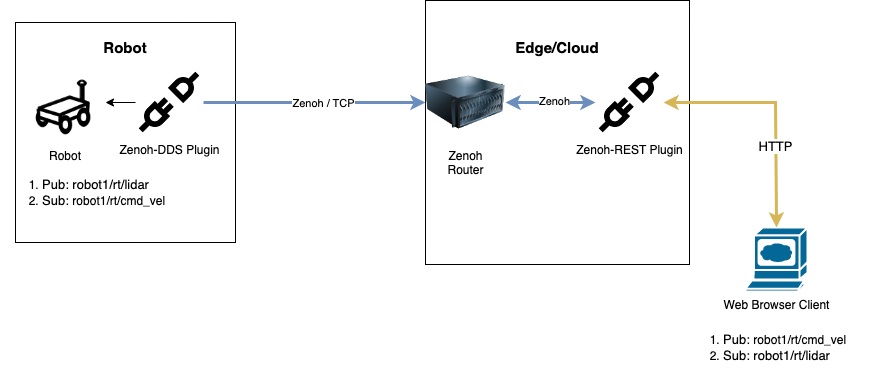
\includegraphics[width=0.95\textwidth]{figures/remote-steuerung.drawio.png}
  \end{center}
  \caption{Robotersteuerung über den Browser}
  \label{fig:Robotersteuerung über den Browser}
\end{figure}

Im vorangegangenen Beispiel sendet der Roboter die Bewegungsdaten über das Topic \code{robot1/rt/lidar} an den den Web Client. Dieser kann die Daten auswerten und darauf über das Topic \code{robot1/rt/cmd\_vel} die Geschwindigkeit anpassen.
Wie man also in \ref{fig:Robotersteuerung über den Browser} erkennen kann, ist die Einbindung von externen Clients mittels dem REST-Protokoll relativ einfach. Dies eröffnet eine weitreichende Möglichkeiten um weitere Endgeräte wie zum Beispiel Smartphones an das \acrlong{cttc} anzubinden.

% subsection Robotersteuerung über den Browser (end)

\subsection{Steuerung über WAN (Internet)} % (fold)
\label{sub:Steuerung über WAN (Internet)}

Entfernte Zugriffe auf Roboter sind wie im letzten Kapitel beschrieben ein wichtiger Use Case für die Robotik. Oftmals sind die Gegebenheiten des Netzwerkes jedoch nicht so optimal wie im vorhergegangenen Beispiel. Vor allem im Bereich des Edge und Cloud Computing muss eine Nachricht verschiedene Netze durchqueren um von einem Sender zu einem Empfänger zu gelangen. Um verschiedene Netze zu durchqueren wird oftmals eine Netzwerk Adressübersetzung, kurz NAT, eingesetzt. Um trotz der verschiedenen Netzüberquerungen einen einfachen Zugriff auf die Roboter zu ermöglichen, muss das genutzte Protokoll diese Gegebenheiten berücksichtigen.\\
Im Folgenden Use Case wird wieder eine entfernte Steuerung eines Roboters beschrieben. Hierbei wird der Fokus jedoch auf die Überbrückung der verschiedenen Netze gelegt.\\

Der Aufbau dieses Use Cases ist von den Komponenten ähnlich wie die beiden vorherigen. Die Steuerung wird in dem Beispiel abstrahiert.\\
Das Ziel an diesem Beispiel ist es einen Roboter von einem entfernten Netzwerk aus zu steuern. Dieses kann sich zum Beispiel geographisch an einem anderen Ort befinden. In \ref{fig:Steuerung über WAN (Internet)} werden zwei Möglichkeiten zur Verbindung betrachtet.\\
Bei der ersten Verbindung handelt es sich um die durchgehende Linie in \ref{fig:Steuerung über WAN (Internet)}. In diesem Fall kann das Netzwerk des Roboters keinen öffentlichen Port, wie zum Beispiel für eine TCP Verbindung öffentlich zur Verfügung stellen. Man braucht also einen externen Server bei der man eine Subscription erstellen kann. Wie in der Abbildung zu sehen, wird dies mit einem einfachen Cloud Server gelöst. Auf diesem läuft ein Zenoh Router, der durch eine öffentliche Adresse zugänglich ist. Sowohl die Steuerung als auch das Zenoh DDS Plugin können dann eine Verbindung mit dem Router im Cloud Server aufbauen. Diese Lösung ist für Anwendungen interessant bei denen man keinen Einfluss auf das Netzwerk hat oder dieses aus Sicherheitsgründen nicht ändern kann.\\
Die Alternative, direkte Verbindung, wird als gestrichene Linie dargestellt. Im Netzwerk des Roboters wird dabei ein Port für die TCP Verbindung geöffnet und die eingehenden Anfragen an das DDS Zenoh Plugin weitergeleitet. Die Steuerung kann dann eine direkte Verbindung zum Plugin aufbauen.\\

\begin{figure}
  \begin{center}
    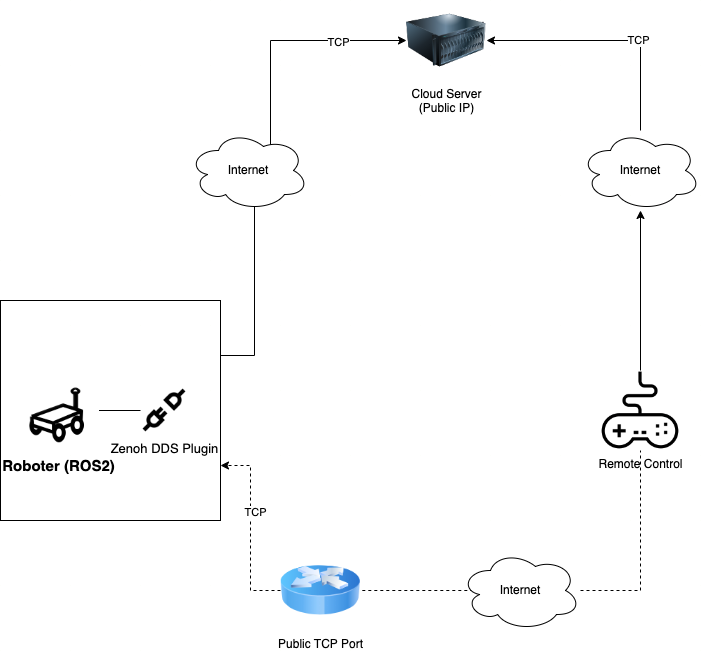
\includegraphics[width=0.6\textwidth]{figures/wan-steuerung.drawio.png}
  \end{center}
  \caption{Steuerung über WAN (Internet)}
  \label{fig:Steuerung über WAN (Internet)}
\end{figure}

Eine wichtige Funktion von verteilten Systemen ist die Ausfallsicherheit. Um dies im oberen Beispiel zu gewährleisten, kann man einen zweiten Zenoh Router in einer weiteren Cloud Instanz einrichten. Diese wird mit der ersten Instanz verbunden. Als Verbindungsparameter werden für die Steuerung und dem Zenoh DDS Router die Adressen beider Server mitgegeben. Im Falle des Ausfalls von einem Server, schalten beide Clients automatisch auf den zweiten Router um.\\
Anhand des letzten Beispiels, kann man eine weitere nützliche Eigenschaft für das \acrlong{cttc} erkennen. Mit Zenoh wird eine Möglichkeit geboten, verschiedene Akteure mittels verschiedenen Protokollen, an geographisch verteilten Orten zu Verbinden ohne einen großen Aufwand im Entwicklungsbereich zu haben.

% subsection Steuerung über WAN (Internet) (end)

% section Cloud und Edge Robotic Use cases (end)
